\documentclass[conference]{IEEEtran}
%\usepackage{cite}
\usepackage[backend=biber,citestyle=ieee]{biblatex}
\usepackage[T1]{fontenc}
\usepackage[utf8]{inputenc}
\usepackage{amsmath, amssymb, amsfonts}
\usepackage{algorithmic}
\usepackage{graphicx}
\usepackage{textcomp}
\usepackage{xcolor}
\usepackage{hyperref}
\addbibresource{report.bib}

\graphicspath{{imgs}}
% What is this?
\def\BibTeX{{\rm B\kern-.05em{\sc i\kern-.025em b}\kern-.08em
    T\kern-.1667em\lower.7ex\hbox{E}\kern-.125emX}}


\begin{document}
\title{Data Science Final Project Report}
\author{\IEEEauthorblockN{Andr\'es Ponce}
		\IEEEauthorblockA{\textit{Department of Computer Science} \\
		\textit{National Cheng Kung University} \\
		Tainan, Taiwan \\
		andresponce@ismp.csie.ncku.edu.tw}
}
%\author{\IEEEauthorblockN{1\textsuperscript{st} Given Name Surname}
%\IEEEauthorblockA{\textit{dept.\ name of organization (of Aff.)} \\
%\emph{name of organization (of Aff.)}\\
%City, Country \\
%email address or ORCID}
%}

\maketitle
\begin{abstract}
	Many e-commerce platforms need to search for similar or identical products
	given some query image.
	Doing so can increase the platform's ability to recommend interesting 
	products or analyze purchasing trends across product categories.
	For the eBay eProduct Visual Search Challenge, participants take a set
	of query images and search a large index set for images of matching products.
	We first train a model to recognize the hierarchical structure of the different
	image categories.
	Then, we use our model's output to produce hashes of the index images
	and query images using locality sensitive hashing, and locate identical products by comparing these hashes.
	This paper describes the motviation, approach, and results of the 
	comptetition.
\end{abstract}

\section{Introduction}
E-commerce platforms continue to grow and play a large role in consumer's
shopping behavior.
Especially with the pandemic, more people relied on such platforms for 
many of their purchases~\cite{jilkova2021digital}.

%PRODUCT PRODUCT PRODUCT %
Platforms where users directly sell their own products especially
benefit from finding images of identical products.
When a user searches for a product, he or she expects the results to contain
images of the same product.
On sites like eBay, identifying identical products can be very useful when 
aggregating sales of different listings of the same product.
Not only do e-commerce platforms rely on such visual search, but also visual
search engines such as Google Images, where the user can use an image as a query
instead of a search term.

The eBay eProduct Visual Recognition Challenge~\cite{jiangbo2021ebay} consists of
finding images of the same product from a large index set of images.
This challenge is one of fine-grained visual classification, since we are trying to 
find images of \emph{the same} product. 
Similar yet non-identical products can differ only by very fine details; likewise,
images of identical products can differ only in lighting conditions or other small
factors, increasing the difficulty of the task.
Despite the possibility for many small changes, our model should be resilient to such 
invariant factors and be able to distinguish similar products from each other.

\section{Competition Description}
Current image datasets do not focus enough on super fine-grained object detection.
This prompted the authors to create the eProduct dataset focusing on fine-grained
visual recognition.
The dataset is divided into training, validation, and query sections. 

The training set consists of around 1.3 million labeled images modelled after the ImageNet~\cite{deng2009imagenet} dataset.
Each image also comes with three levels of hierarchical labels: its meta class (16 total), level 2 class (17 total),
and the leaf class (1,000 total) as well as the product title and a unique identifier.
Also like ImageNet, the validation set contains 50,000 images, each containing the same information 
for each image as the training set.

The testing set contains 10,000 query images with only the unqiue identifier.
Given one of these query images, our task is to search for identical products to this query in a 1.1 million image index set, also provided
as part of the testing set.
The index set contains \emph{groundtruth sets} which are a match with any of the query images and 
a \emph{distractor set} which does not match with any query image.
Fig.~\ref{fig:structure} describes the structure of the dataset and the challenge posed by similar products.

\section{Related Work}

\begin{figure}[!t]
\centering
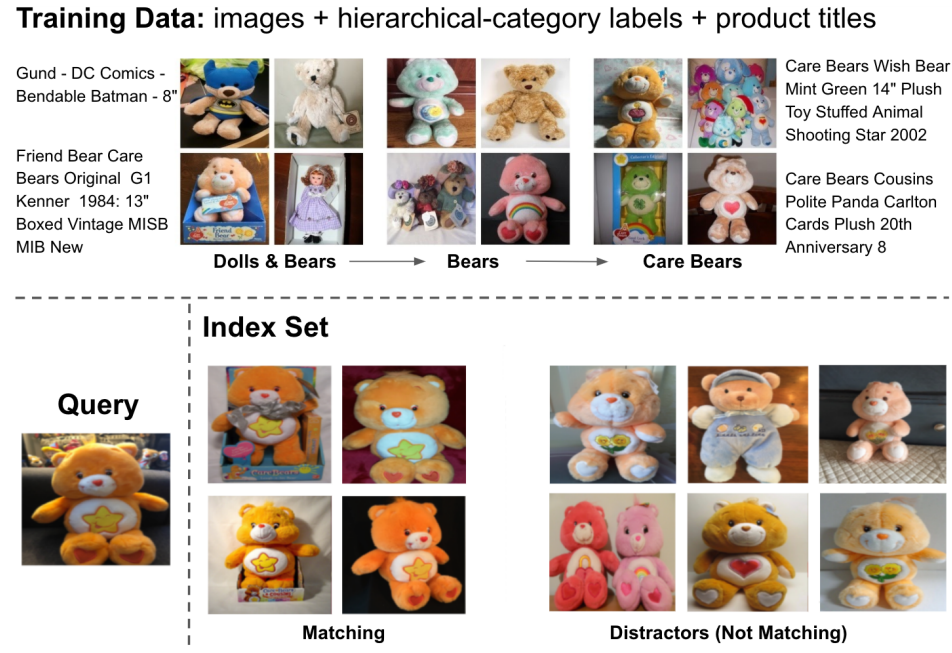
\includegraphics[scale=0.25]{structure}
\caption{eProduct dataset structure. The top section contains a sample training image and the meta,
level 2, and leaf categories. Each level contains a more specific type of product, and the leaf category
can still contain slightly different, non-matching products. 
The bottom section shows the query image and the identical products from the index set, along with a set 
of \emph{distractor} products that do not match with any query image.
Source:~\cite{jiangbo2021ebay}}

\label{fig:structure}
\end{figure}

\section{Method Description}
The visual search problem can be divided into two major parts: training a deep model
to obtain $z$ and calculating the similarity between $z$ and the items in the index set.
We train a deep model for the first part and use locality sensitive hashing to find the 
similarities.

\begin{figure}[!t]
	\centering
	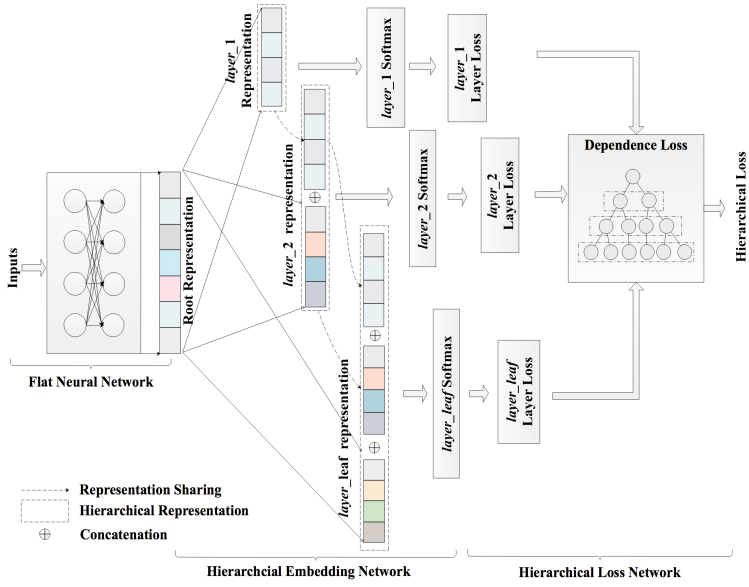
\includegraphics[scale=0.30]{network}
	\caption{Deep Hierarchical Embedding's structure . 
	The network first generates a representation for each hierarchical layer which is the concatenation
	of the prevoius layer's representation and the current layer. Then we calculate the loss
	function for each layer's prediction and use this to calculate dependence and hierarchical loss.
	Source:~\cite{gao2020deep}}
	\label{fig:network}
\end{figure}
\subsection{Deep Learning Model}
The idea behind using a deep model is to obtain a vector $z$ that captures the important
information of an image.
The contents of the vector should be informed not only by the image contents, but also the 
hierarchical descriptions given as part of the training data.
Since there are three hierarchical levels of information (meta class, level 2, leaf categories),
our model should produce similar embeddings for products in similar categories.
This means our model should incorporate this information in some way during training.

However, the categories are not independent of each other.
For example, if a product belongs to a certain meta category, 
there is only a subset of child level 2 categories, and similar for 
child classes.
Our model should take these parent-child relationships into account.

We based our work on Deep Hierarchical Classification~\cite{gao2020deep}, since this model seemed 
specifically designed for hierarchical e-commerce classification.
The architecture contains a flat neural network(FNN) $f(\theta)$ which generates a representation 
for each hierarchical layer $R'_l$. 
This representation is the concatenation of the previous hierarchical layer's representation
$R_l = R_{l-1}\oplus R'_l$ for $ l\neq 1$. 
The first layer's represnetation is not concatenated with anything else.
Each layer's representation is passed through the softmax activation function.

The model contains two loss functions: the layer loss and dependence loss.
Our model attempts to predict the three class levels for each image.

\subsection{Locality Sensitive Hashing}
\section{Training and Experiments}
 \printbibliography
\end{document}
